\chapter{Adaptive Resonance Theory}
ART networks are self-organizing networks that have been able to solve the \emph{stability-plasticity} dilemma. ART able to \emph{switch modes} between plastic and stable without damage to previous learned weight values.

\begin{description}
\item[Stability-plasticity dilemma] not able to learn new information on top of old
\item[Plasticity] for the integration of new knowledge
\item[Stability] to prevent the forgetting of previous knowledge
\end{description}

\section{ART-1}
Designed to cluster and recognize binary patterns only.
\begin{figure}[!h]
\centering
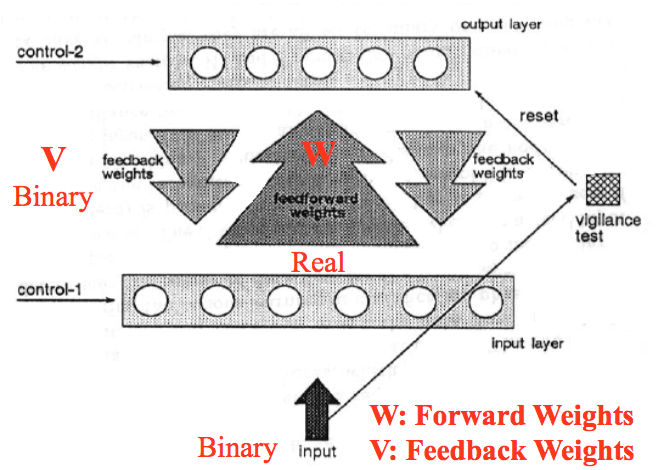
\includegraphics[width=8cm]{chapter10_1}
\end{figure}

\noindent The feed-forward weight matrix is:
$$\mathbf{W} = [\mathbf{w}_1 \mathbf{w}_2 \ldots \mathbf{w}_M]^{T}$$
The feedback weight vector is:
$$\mathbf{V} = [\mathbf{v}_1 \mathbf{v}_2 \ldots \mathbf{v}_N]^{T}$$
The feed-forward weight is proportional to the corresponding feedback weight value:
$$w_{ji} \propto v_{ij}$$
\begin{center} where $v_{ij} \in {0,1}$ and $w_{ji} \in [0,1]$\end{center}
Output layer is a \emph{winner-take-all} layer

\subsubsection{Control Signals of the Network}
$$
control1 = 
\begin{cases}
0 & comparison\ mode \\
1 & input\ mode
\end{cases}
$$

$$
control2 = 
\begin{cases}
0 & failed\ vigilance\ test \\
1 & satisfied\ vigilance\ test
\end{cases}
$$

\subsubsection{Vigilance Test}
Similarity between input pattern $\mathbf{X}$ and feedback pattern $\mathbf{V}_j$:
$$s_j = \frac{|\mathbf{X} \cap \mathbf{V}_j|}{| \mathbf{X} |}$$
Vigilance test is satisfied if $s_j$ is greater than vigilance value $\rho$

\section{ART-1 Algorithm}
\subsubsection{Step 1: Initialization}
Initialize vigilance threshold $\rho$, feed-forward weights $w_{ij}$, and feedback weights $v_{j1}$:
$$0 \le \rho \le 1$$
$$w_{ij} = \frac{1}{1+N}$$
$$v_{ji} = 1$$
\subsubsection{Step 2: The total synaptic input}
\begin{equation*}
\begin{split}
\mathbf{u}_j &= \sum_{i=1}^{n} w_{ji} x_i \\
&= \frac{|\mathbf{V}_j \cap \mathbf{X}|}{0.5 + |\mathbf{V}_j|} \\
& \propto | \mathbf{V}_j \cap \mathbf{X}_i |
\end{split}
\end{equation*}
\begin{center}Since $w_{ji} \propto v_{ij}$ \end{center}

\subsubsection{Step 3: The winner $m$}
$$m = arg\!\max_{j=1...M} u_j\ for\ y_j \ne 0$$
The output
$$
y_j = 
\begin{cases}
1 & j = m \\
0 & j \ne m
\end{cases}
$$
\subsubsection{Step 4: Calculate similarity}
$$s_j = \frac{|\mathbf{X} \cap \mathbf{V}_m |}{| \mathbf{X} |}$$
If $s \ge \rho$, go to step 5. \\
Else if the top-later has any active nodes left, go to step 6. \\
Else, go to step 5 to create a new cluster.
\subsubsection{Step 5: Update the weights of winning node}
$$\mathbf{V}_m^{new} = \mathbf{V}_m \cap \mathbf{X}$$
$$\mathbf{w}_m^{new} = \frac{\mathbf{V}_m^{new}}{0.5 + | \mathbf{V}_m^{new} |}$$
Go to step 2.
\subsubsection{Step 6: Continue search}
Setting output $y_m = 0$. \\
Go to step 3 to find a new winner $m$
